\section{Theoretical Analysis}
\label{sec:analysis}

In this section, the circuit shown in Figure~\ref{fig:t1systemanalysis.pdf} is analysed
theoretically, in terms of its current and voltage.
In analyzing a circuit using Kirchhoff's circuit laws, one can either do nodal analysis using Kirchhoff's current law (KCL) or mesh analysis using Kirchhoff's voltage law (KVL).
In the subsections bellow we explain how the two methods ... in solving the circuit. 



IMPRIME ISTO

\begin{center}
\begin{figure}
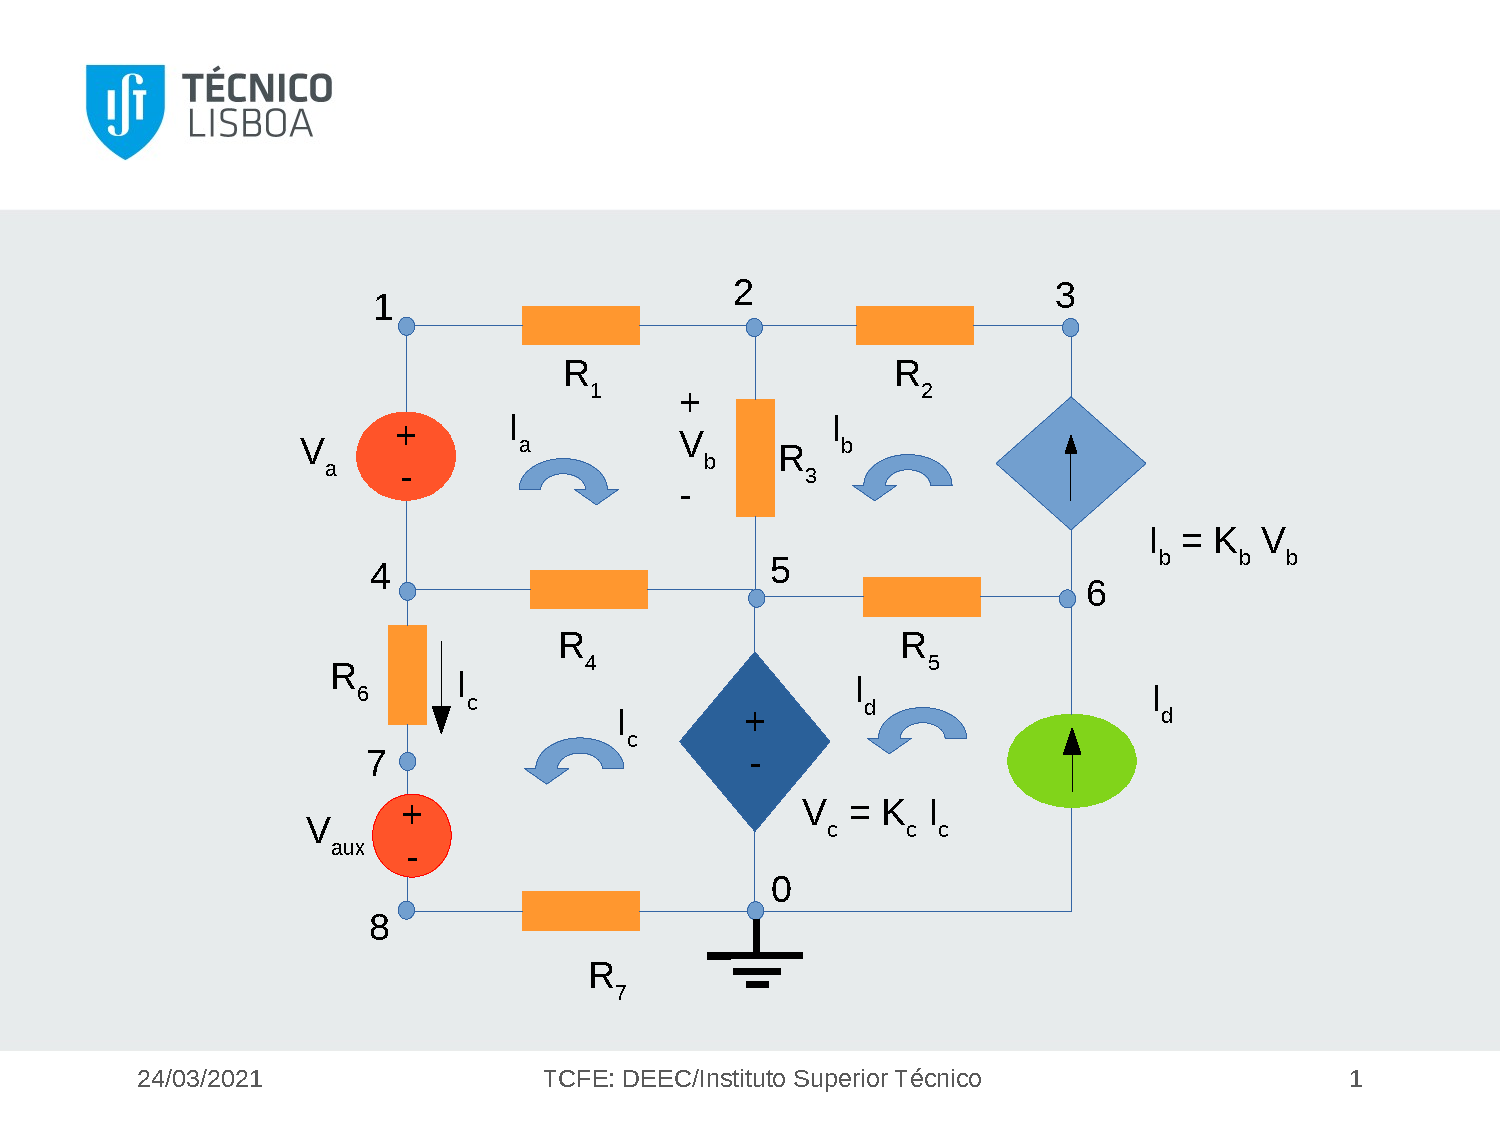
\includegraphics[width  = 10cm]{t1systemanalysis.pdf}
\end{figure}
\end{center}

IMPRIME ISTO


\subsection{Nodal analysis}
The nodal analysis or the branch current method is a method of determining the voltage (potential difference) between "nodes" (points where elements or branches connect) in an electrical circuit in terms of the branch currents. 
Nodal analysis writes an equation at each electrical node, requiring that the branch currents incident at a node must sum to zero.
Since there are 8 nodes in total in this circuit we must have 8 equations in order to find all the 8 voltages.


$\begin{pmatrix}
1 & 0 & 0 & -1 & 0 & 0 & 0 \\
0 & -G2-Kb & G2 & 0 & Kb & 0 & 0 \\
-G1 & G1+G2+G3 & -G2 & 0 & -G3 & 0 & 0 \\
0 & Kb & 0 & 0 & -G5-Kb & G5 & 0 \\
0 & 0 & 0 & -Kc*G6 & 1 & 0 & Kc*G6 \\
0 & 0 & 0 & -G6 & 0 & 0 & G6+G7 \\
0 & 0 & 0 & -G6 & 0 & 0 & G6+G7 
\end{pmatrix}$
$\begin{pmatrix}
V1\\
V2\\
V3\\
V4\\
V5\\
V6\\
V7
\end{pmatrix}$
=
$\begin{pmatrix}
Va\\
0\\
0\\
Id\\
0\\
0\\
0
\end{pmatrix}$


The following table displays the various solutions to the :

\begin{table}[ht]
\centering
\begin{tabular}{c|c} 
 \hline
 BAMUS\\ [0.5ex] 
 \hline\hline
V1 & 8.194795e+00 V\\ \hline
V2 & 7.917828e+00 V\\ \hline
V3 & 7.340169e+00 V\\ \hline
V4 & 2.978754e+00 V\\ \hline
V5 & 7.957540e+00 V\\ \hline
V6 & 1.197664e+01 V\\ \hline
V7 & 9.776608e-01 V\\ \hline
V8 & 0.000000e+00 V\\ \hline 
\end{tabular}
\caption{Table ...}
\label{table:2}
\end{table}

o q da cada um teoricamente

\subsection{Mesh analysis}

Mesh analysis is a method that is used to solve circuits for the currents at any place in the electrical circuit.\\
This analysis makes use of Kirchhoff’s voltage law to arrive at a set of equations guaranteed to be solvable if the circuit has a solution.\\In this case, we use four equations in order to find the four circulation currents, since we have four elementar meshes in this circuit.

$\begin{pmatrix}
R1+R3+R4 & R3 & R4 & 0 \\
Kb*R3 & Kb*R3 - 1 & 0 & 0 \\
R4 & 0 & R4+R6+R7-Kc & 0 \\
0 & 0 & 0 & 1 
\end{pmatrix}$
$\begin{pmatrix}
Ia\\
Ib\\
Ic\\
Id
\end{pmatrix}$
=
$\begin{pmatrix}
Va\\
0\\
0\\
Id
\end{pmatrix}$


The following table is the info that was already given to us:

\begin{table}[ht]
\centering
\begin{tabular}{c|c} 
 \hline
 BAMUS\\ [0.5ex] 
 \hline\hline
Ia & 2.732478e-01 mA\\ \hline
Ib & -2.864551e-01 mA\\ \hline
Ic & 9.563162e-01 mA\\ \hline
Id & 1.029587e+00 mA\\ \hline 
\end{tabular}
\caption{Table ...}
\label{table:3}
\end{table}


o que da cada um teoricamente















